\documentclass[12pt,twoside]{article}
\usepackage[dvipsnames]{xcolor}
\usepackage{tikz,graphicx,amsmath,amsfonts,amscd,amssymb,bm,cite,epsfig,epsf,url}
\usepackage[hang,flushmargin]{footmisc}
\usepackage[colorlinks=true,urlcolor=blue,citecolor=blue]{hyperref}
\usepackage{amsthm,multirow,wasysym,appendix}
\usepackage{array,subcaption} 
% \usepackage[small,bf]{caption}
\usepackage{bbm}
\usepackage{pgfplots}
\usetikzlibrary{spy}
\usepgfplotslibrary{external}
\usepgfplotslibrary{fillbetween}
\usetikzlibrary{arrows,automata}
\usepackage{thmtools}
\usepackage{blkarray} 
\usepackage{textcomp}
\usepackage[left=0.8in,right=1.0in,top=1.0in,bottom=1.0in]{geometry}


\usepackage{times}
\usepackage{amsfonts}
\usepackage{amsmath}
\usepackage{latexsym}
\usepackage{color}
\usepackage{graphics}
\usepackage{enumerate}
\usepackage{amstext}
\usepackage{blkarray}
\usepackage{url}
\usepackage{epsfig}
\usepackage{bm}
\usepackage{hyperref}
\hypersetup{
    colorlinks=true,
    linkcolor=blue,
    filecolor=magenta,      
    urlcolor=blue,
}
\usepackage{textcomp}
\usepackage[left=0.8in,right=1.0in,top=1.0in,bottom=1.0in]{geometry}
\usepackage{mathtools}
\usepackage{minted}



%% Probability operators and functions
%
% \def \P{\mathrm{P}}
\def \P{\mathrm{P}}
\def \E{\mathrm{E}}
\def \Var{\mathrm{Var}}
\let\var\Var
\def \Cov {\mathrm{Cov}} \let\cov\Cov
\def \MSE {\mathrm{MSE}} \let\mse\MSE
\def \sgn {\mathrm{sgn}}
\def \R {\mathbb{R}}
\def \C {\mathbb{C}}
\def \N {\mathbb{N}}
\def \Z {\mathbb{Z}}
\def \cV {\mathcal{V}}
\def \cS {\mathcal{S}}
\DeclareMathOperator*{\argmin}{arg\,min}
\DeclareMathOperator*{\argmax}{arg\,max}
\newcommand{\red}[1]{\textcolor{red}{#1}}
\newcommand{\blue}[1]{\textcolor{blue}{#1}}
\newcommand{\green}[1]{\textcolor{ForestGreen}{ #1}}
\newcommand{\fuchsia}[1]{\textcolor{RoyalPurple}{ #1}}

%
%% Probability distributions
%
%\def \Bern    {\mathrm{Bern}}
%\def \Binom   {\mathrm{Binom}}
%\def \Exp     {\mathrm{Exp}}
%\def \Geom    {\mathrm{Geom}}
%\def \Norm    {\mathcal{N}}
%\def \Poisson {\mathrm{Poisson}}
%\def \Unif    {\mathrm {U}}
%
\newcommand{\bdb}[1]{\textcolor{red}{#1}}

\newcommand{\ml}[1]{\mathcal{ #1 } }
\newcommand{\wh}[1]{\widehat{ #1 } }
\newcommand{\wt}[1]{\widetilde{ #1 } }
\newcommand{\conj}[1]{\overline{ #1 } }
\newcommand{\rnd}[1]{\tilde{ #1 } }
\newcommand{\rv}[1]{ \rnd{ #1}  }
\newcommand{\rx}{\rnd{ x}  }
\newcommand{\ry}{\rnd{ y}  }
\newcommand{\ra}{\rnd{ a}  }
\newcommand{\rb}{\rnd{ b}  }
\newcommand{\rpc}{\widetilde{ pc}  }

\def \cnd {\, | \,}
\def \Id { I }
\def \J {\mathbf{1}\mathbf{1}^T}

\newcommand{\op}[1]{\operatorname{#1}}
\newcommand{\setdef}[2]{ := \keys{ #1 \; | \; #2 } }
\newcommand{\set}[2]{ \keys{ #1 \; | \; #2 } }
\newcommand{\sign}[1]{\op{sign}\left( #1 \right) }
\newcommand{\trace}[1]{\op{tr}\left( #1 \right) }
\newcommand{\tr}[1]{\op{tr}\left( #1 \right) }
\newcommand{\inv}[1]{\left( #1 \right)^{-1} }
\newcommand{\abs}[1]{\left| #1 \right|}
\newcommand{\sabs}[1]{| #1 |}
\newcommand{\keys}[1]{\left\{ #1 \right\}}
\newcommand{\sqbr}[1]{\left[ #1 \right]}
\newcommand{\sbrac}[1]{ ( #1 ) }
\newcommand{\brac}[1]{\left( #1 \right) }
\newcommand{\bbrac}[1]{\big( #1 \big) }
\newcommand{\Bbrac}[1]{\Big( #1 \Big)}
\newcommand{\BBbrac}[1]{\BIG( #1 \Big)}
\newcommand{\MAT}[1]{\begin{bmatrix} #1 \end{bmatrix}}
\newcommand{\sMAT}[1]{\left(\begin{smallmatrix} #1 \end{smallmatrix}\right)}
\newcommand{\sMATn}[1]{\begin{smallmatrix} #1 \end{smallmatrix}}
\newcommand{\PROD}[2]{\left \langle #1, #2\right \rangle}
\newcommand{\PRODs}[2]{\langle #1, #2 \rangle}
\newcommand{\der}[2]{\frac{\text{d}#2}{\text{d}#1}}
\newcommand{\pder}[2]{\frac{\partial#2}{\partial#1}}
\newcommand{\derTwo}[2]{\frac{\text{d}^2#2}{\text{d}#1^2}}
\newcommand{\ceil}[1]{\lceil #1 \rceil}
\newcommand{\Imag}[1]{\op{Im}\brac{ #1 }}
\newcommand{\Real}[1]{\op{Re}\brac{ #1 }}
\newcommand{\norm}[1]{\left|\left| #1 \right|\right| }
\newcommand{\norms}[1]{ \| #1 \|  }
\newcommand{\normProd}[1]{\left|\left| #1 \right|\right| _{\PROD{\cdot}{\cdot}} }
\newcommand{\normTwo}[1]{\left|\left| #1 \right|\right| _{2} }
\newcommand{\normTwos}[1]{ \| #1  \| _{2} }
\newcommand{\normZero}[1]{\left|\left| #1 \right|\right| _{0} }
\newcommand{\normTV}[1]{\left|\left| #1 \right|\right|  _{ \op{TV}  } }% _{\op{c} \ell_1} }
\newcommand{\normOne}[1]{\left|\left| #1 \right|\right| _{1} }
\newcommand{\normOnes}[1]{\| #1 \| _{1} }
\newcommand{\normOneTwo}[1]{\left|\left| #1 \right|\right| _{1,2} }
\newcommand{\normF}[1]{\left|\left| #1 \right|\right| _{\op{F}} }
\newcommand{\normLTwo}[1]{\left|\left| #1 \right|\right| _{\ml{L}_2} }
\newcommand{\normNuc}[1]{\left|\left| #1 \right|\right| _{\ast} }
\newcommand{\normOp}[1]{\left|\left| #1 \right|\right|  }
\newcommand{\normInf}[1]{\left|\left| #1 \right|\right| _{\infty}  }
\newcommand{\proj}[1]{\mathcal{P}_{#1} \, }
\newcommand{\diff}[1]{ \, \text{d}#1 }
\newcommand{\vc}[1]{\boldsymbol{\vec{#1}}}
\newcommand{\rc}[1]{\boldsymbol{#1}}
\newcommand{\vx}{\vec{x}}
\newcommand{\vy}{\vec{y}}
\newcommand{\vz}{\vec{z}}
\newcommand{\vu}{\vec{u}}
\newcommand{\vv}{\vec{v}}
\newcommand{\vb}{\vec{\beta}}
\newcommand{\va}{\vec{\alpha}}
\newcommand{\vaa}{\vec{a}}
\newcommand{\vbb}{\vec{b}}
\newcommand{\vg}{\vec{g}}
\newcommand{\vw}{\vec{w}}
\newcommand{\vh}{\vec{h}}
\newcommand{\vnu}{\vec{\nu}}
\newcommand{\rvnu}{\vc{\nu}}

\newtheorem{theorem}{Theorem}[section]
% \declaretheorem[style=plain,qed=$\square$]{theorem}
\newtheorem{corollary}[theorem]{Corollary}
\newtheorem{definition}[theorem]{Definition}
\newtheorem{lemma}[theorem]{Lemma}
\newtheorem{remark}[theorem]{Remark}
\newtheorem{algorithm}[theorem]{Algorithm}

% \theoremstyle{definition}
%\newtheorem{example}[proof]{Example}
%\declaretheorem[style=definition,qed=$\triangle$,sibling=definition]{example}
%\declaretheorem[style=definition,qed=$\bigcirc$,sibling=definition]{application}

%
%% Typographic tweaks and miscellaneous
%\newcommand{\sfrac}[2]{\mbox{\small$\displaystyle\frac{#1}{#2}$}}
%\newcommand{\suchthat}{\kern0.1em{:}\kern0.3em}
%\newcommand{\qqquad}{\kern3em}
%\newcommand{\cond}{\,|\,}
%\def\Matlab{\textsc{Matlab}}
%\newcommand{\displayskip}[1]{\abovedisplayskip #1\belowdisplayskip #1}
%\newcommand{\term}[1]{\emph{#1}}
%\renewcommand{\implies}{\;\Rightarrow\;}

% My macros

\def\Kset{\mathbb{K}}
\def\Nset{\mathbb{N}}
\def\Qset{\mathbb{Q}}
\def\Rset{\mathbb{R}}
\def\Sset{\mathbb{S}}
\def\Zset{\mathbb{Z}}
\def\squareforqed{\hbox{\rlap{$\sqcap$}$\sqcup$}}
\def\qed{\ifmmode\squareforqed\else{\unskip\nobreak\hfil
\penalty50\hskip1em\null\nobreak\hfil\squareforqed
\parfillskip=0pt\finalhyphendemerits=0\endgraf}\fi}

%\DeclareMathOperator*{\E}{\rm E}
%\DeclareMathOperator*{\argmax}{\rm argmax}
%\DeclareMathOperator*{\argmin}{\rm argmin}
%\DeclareMathOperator{\sgn}{sign}
\DeclareMathOperator{\supp}{supp}
\DeclareMathOperator{\last}{last}
%\DeclareMathOperator{\sign}{\sgn}
\DeclareMathOperator{\diag}{diag}
\providecommand{\abs}[1]{\lvert#1\rvert}
\providecommand{\norm}[1]{\lVert#1\rVert}
\def\vcdim{\textnormal{VCdim}}
\DeclareMathOperator*{\B}{\textbf{B}}

%\DeclarePairedDelimiter\ceil{\lceil}{\rceil}
%\DeclarePairedDelimiter\floor{\lfloor}{\rfloor}

\newcommand{\cX}{{\mathcal X}}
\newcommand{\cY}{{\mathcal Y}}
\newcommand{\cA}{{\mathcal A}}
\newcommand{\ignore}[1]{}
\newcommand{\bi}{\begin{itemize}}
\newcommand{\ei}{\end{itemize}}
\newcommand{\be}{\begin{enumerate}}
\newcommand{\ee}{\end{enumerate}}
\newcommand{\bd}{\begin{description}}
\newcommand{\ed}{\end{description}}
\newcommand{\h}{\widehat}
\newcommand{\e}{\epsilon}
\newcommand{\mat}[1]{{\mathbf #1}}
%\newcommand{\R}{\mat{R}}
\newcommand{\0}{\mat{0}}
\newcommand{\M}{\mat{M}}

\newcommand{\D}{\mat{D}}
\renewcommand{\r}{\mat{r}}
\newcommand{\x}{\mat{x}}
\renewcommand{\u}{\mat{u}}
\renewcommand{\v}{\mat{v}}
\newcommand{\w}{\mat{w}}
\renewcommand{\H}{\text{0}}
\newcommand{\T}{\text{1}}
%\newcommand{\set}[1]{\{#1\}}
\newcommand{\xxi}{{\boldsymbol \xi}}
\newcommand{\ssigma}{{\boldsymbol \sigma}}
\newcommand{\Alpha}{{\boldsymbol \alpha}}
\newcommand{\tts}{\tt \small}
\newcommand{\hint}{\emph{hint}}
\newcommand{\matr}[1]{\bm{#1}}     % ISO complying version
\newcommand{\vect}[1]{\bm{#1}} % vectors

%\newcommand{\Var}{\mathrm{Var}}
%\newcommand{\Cov}{\mathrm{Cov}}

% New commands
\newcommand{\SP}{\mathbf{S}_{+}^n}
\newcommand{\Proj}{\mathcal{P}_{\mathcal{S}}}
\DeclarePairedDelimiterX{\inp}[2]{\langle}{\rangle}{#1, #2}
\newtheorem{proof}{Proof}


\begin{document}

\begin{center}
{\large{\textbf{Homework 11}} } \vspace{0.2cm}\\
Due May 10 at 11 pm
\end{center}
Yves Greatti - yg390\\

\begin{enumerate}

\item (Lasso and $\ell_0$)
The file \texttt{X.txt} contains a $50 \times 300$ matrix $X$,
  and the file \texttt{y.txt} contains the $50\times 1$ vector
  $y$.  Each line of each file represents a row of the corresponding
  matrix, and the values on each line are space-delimited.
  \begin{enumerate}
  \item Consider the lasso problem
    $$\min_{\beta} \frac{1}{2n}\|X\beta -y\|^2 + \lambda\|\beta\|_1$$
    where $\lambda>0$ is a parameter and $n=50$.  Construct a (semilogx) plot
    that draws a
    separate path for each coefficient value as a function
    of~$\lambda$.
    Include values of $\lambda$ between $0.01$ and $2$ (you can
    include more if you want),
    and make your values spaced evenly on the log axis (e.g.,
    \texttt{np.geomspace}).  You can solve the lasso problem using

    whatever code/library you want.\\
   	\begin{figure}[H]
		\centering
		\captionsetup{justification=centering}
		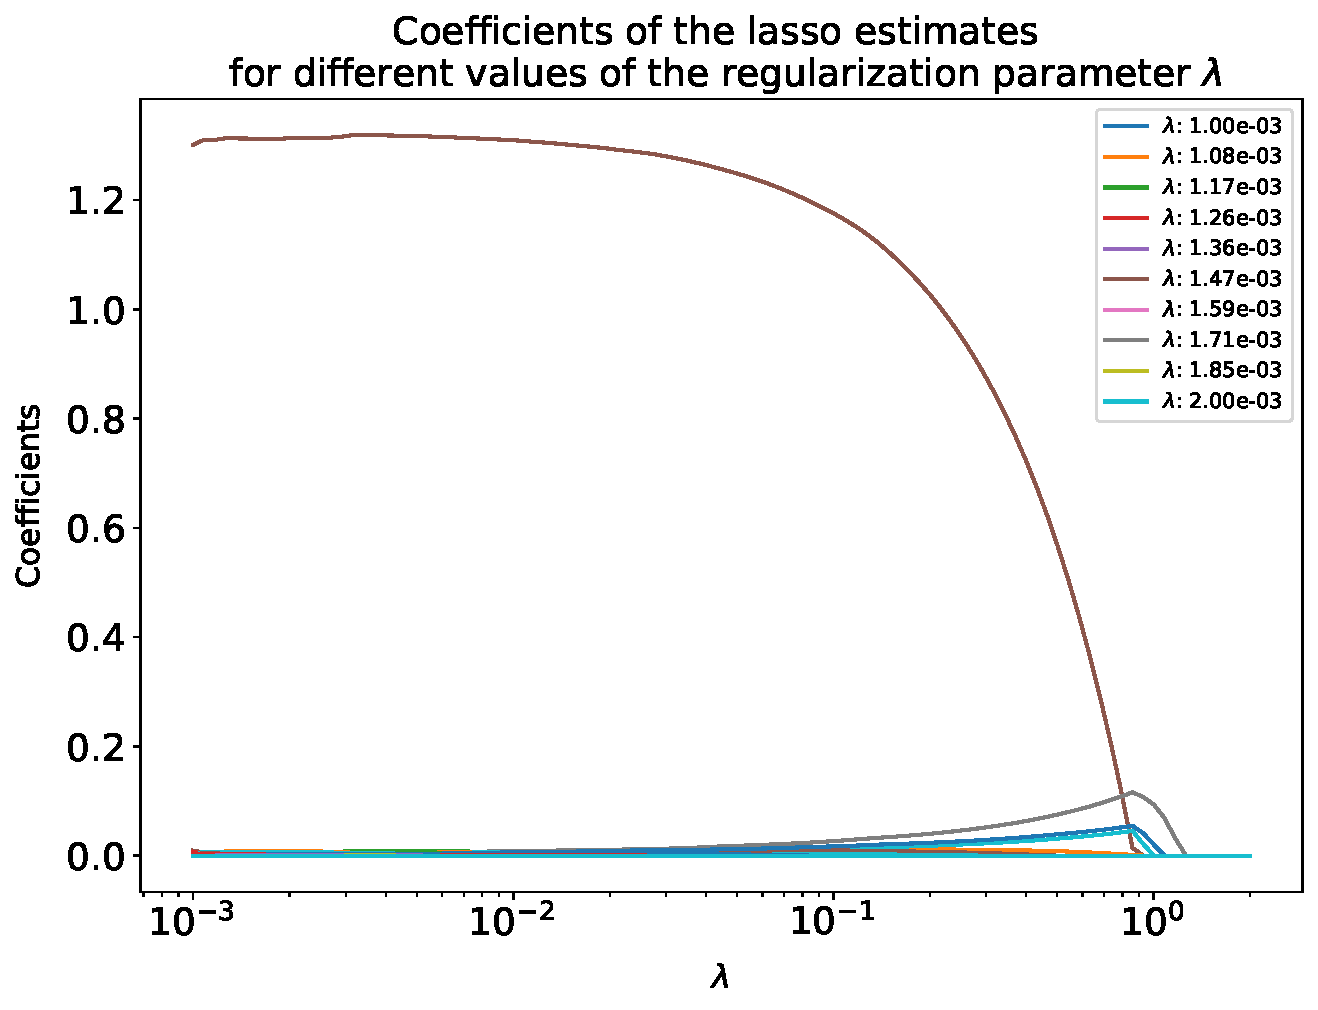
\includegraphics[width=200pt]{code/lasso_vs_lo/lasso.pdf}
	\end{figure}
 
  \item Determine the minimizer of
    $$\begin{array}{ll}
    \text{minimize} & \|\beta\|_0\\
    \text{subject to} & X\beta = y.
    \end{array}$$
    
    Assume that the minimizer has small $\ell_0$ norm, i.e $\ell_0 \leq 2$. Explain your strategy and justify that it finds the minimizer.  
    Report the nonzero coefficients of the minimizer, and
    their values.  Remember that two floating point values may be different for numerical reasons even if they represent the same value.
    \item Will your strategy in (b) always find the optimal minimizer of any least-squares problem with $\ell_0$ regularization?
  \end{enumerate}
  
 \newpage
 \item (Proximal operator) The proximal operator of a function $f: \R^n \rightarrow \R$ is defined as
\begin{align}
\op{prox}_{f}\brac{y} := \arg \min_{x} f\brac{x}+ \frac{1}{2} \normTwo{x-y}^2.
\end{align}
  \begin{enumerate}
  \item Derive the proximal operator of the squared $\ell_2$ norm weighted by a constant $\alpha > 0$, i.e. $f(x)=\alpha \normTwo{x}^2$.

\begin{align*}
\op{prox}_{f}\brac{y} := \arg \min_{x}  \alpha \normTwo{x}^2 + \frac{1}{2} \normTwo{x-y}^2
\end{align*}

The two terms are quadratic, therefore differentiable, the gradient is 
$$
	\nabla_x \op{prox}_{f}\brac{y} = 2 \alpha x + (x-y)
$$
 Setting the gradient to zero, yields:
\begin{align*}
	2 \alpha x + (x-y)			&= 	0 \\
		x 					&= \frac{1} {1+2 \alpha} y \\
		\op{prox}_{f}\brac{y} 		&=	 \frac{1} {1+2 \alpha} y, \alpha > 0 \\
\end{align*}
 
  \item Prove that the proximal operator of the $\ell_1$ norm weighted by a constant $\alpha > 0$ is a soft-thresholding operator,
\begin{align}
\op{prox}_{\alpha \, \normOne{ \cdot }}\brac{ y } & = \ml{S}_{\alpha}\brac{y},
\end{align}
where 
\begin{align}
\ml{S}_{\alpha}\brac{y}[i] := 
\begin{cases}
y\,[i] - \op{sign}\brac{y\,[i]} \alpha  \qquad & \text{if $\abs{y\,[i]} \geq \alpha$}, \\
0 \quad & \text{otherwise}.
\end{cases}
\end{align}\\

$$
\op{prox}_{\alpha \, \normOne{ \cdot }}\brac{ y } = \alpha \|x\|_1 + \frac{1}{2} \normTwo{x-y}^2, \alpha > 0
$$
And we are looking for:
\begin{align*}
	0 \in \partial( \alpha \|x\|_1) + \nabla_x (\frac{1}{2} \normTwo{x-y}^2) \\
	0 \in \alpha \; \partial( \|x\|_1) + (x-y) \\
\end{align*}
We examine each component of $x$ and $y$ separately.
Assume first that $x[i] \neq 0$ then $ \partial( \|x\|_1) = \sign{x[i]}$, setting the subgradient to $0$, we have:
\begin{align*}
	x[i] - y[i] + \alpha \sign{x[i]}	&= 0 \\
	x[i]					&= y[i] - \alpha \sign{x[i]} \\
\end{align*}
Note that
\begin{align*}
	x[i] < 0, \sign{x[i]} = -1 &\rightarrow y[i] + \alpha < 0 \text{ ~ or }  y[i] < -\alpha < 0 \\
	x[i] > 0, \sign{x[i]} = 1 &\rightarrow y[i] - \alpha > 0 \text{ ~ or }  y[i] > \alpha > 0 \\
\end{align*}
thus in this case $\sign{x[i]} = \sign{y[i]}$ and the optimal point is $y[i] - \alpha \sign{y[i]}$.
In the case where $x[i]=0$, let $\gamma =  \partial(\|x\|_1), | \gamma | \le 1$ then it holds
\begin{align*}
	x[i] - y[i] + \alpha \gamma = 0 &\rightarrow y[i] - \alpha \gamma = 0 \\
							&	y[i] = \gamma \alpha \\
							& |y[i]| \le \alpha
\end{align*}
Putting all together, we get
\begin{align}
\op{prox}_{\alpha \, \normOne{ \cdot }}\brac{ y } = 
\begin{cases}
y\,[i] - \op{sign}\brac{y\,[i]} \alpha  \qquad & \text{if $\abs{y\,[i]} \geq \alpha$}, \\
0 \quad & \text{otherwise}.
\end{cases}
\end{align}

    \item Prove that if $X \in \R^{p \times n}$ has orthonormal rows ($p \leq n$) and $y \in \R^{n}$, then for any function $f$
\begin{align}
\arg \min_{\beta} \frac{1}{2} \normTwo{ y - X^T\beta }^2 + f(\beta) = \arg \min_{\beta} \frac{1}{2} \normTwo{ Xy - \beta }^2 + f(\beta).
\end{align}
The two expressions for the same function $f$ differs on the first term, so we want to show that
$$
\arg \min_{\beta} \normTwo{ y - X^T\beta }^2  =  \arg \min_{\beta} \normTwo{ Xy - \beta }^2
$$
$X$ having orthonormal rows: $X X^T = I$, and
\begin{align*}
	\normTwo{ y - X^T\beta }^2  	&= (y^T -\beta^T X) (y - X^T\beta) \\
						  	&= y^T y - y^T X^T \beta - \beta^T X y + \beta^T X X^T \beta \\
						  	&=   y^T y - y^T X^T \beta - \beta^T X y +  \beta^T \beta \\
	 \normTwo{ Xy - \beta }^2 		&= (y^T X^T - \beta^T) (Xy - \beta) \\
	 						&= y^T X^T X y - y^T X^T \beta - \beta^T X y +  \beta^T \beta \\
	\normTwo{ y - X^T\beta }^2  	&= 	 \normTwo{ Xy - \beta }^2 \\					
\end{align*}

\item Use the answers to the previous questions to compare the ridge-regression and lasso estimators for a regression problem where the features are orthonormal.
  \end{enumerate}
The use of $l_1$, $l_2$ norms gives rise to the problems, for $\lambda > 0$:

\begin{align*}
\frac{1}{2} \argmin_\beta \| y - X^T \beta\|_2^2 + \lambda \|\beta\|_2^2	& \text{~ Ridge regression} \\
\frac{1}{2} \argmin_\beta \| y - X^T \beta\|_2^2 + \lambda \|\beta\|_1	& \text{~ Lasso regression}
\end{align*} 
which is equivalent from part c) to
\begin{align*}
 \argmin_\beta  \lambda \|\beta\|_2^2 + \frac{1}{2} \| \beta - X y \|_2^2 	& \text{~ Ridge regression} \\
 \argmin_\beta   \lambda \|\beta\|_1+    \frac{1}{2} \| \beta - X y \|_2^2 	& \text{~ Lasso regression}
\end{align*} 
From part a) and b), the solutions of these two problems are the proximal operators:
\begin{align*}
	\beta_{\text{ridge}}	&= 	 \frac{1} {1+2 \lambda} X y \\
	\beta_{\text{lasso}}	&= 	  \ml{S}_{\lambda}\brac{X y}\\
\end{align*} 
We see that the lasso solution shows sparsity: when the component wise least-square coefficients, $X y$, are not small they are shrunken towards $0$ by $\lambda$, and set to $0$ when they are small.
In contrast the ridge regression estimates are never sparse, all scaled with a single factor inversely proportional to $\lambda$.
 
 \newpage
  \item (Proximal gradient method)   
 \begin{enumerate}
 \item The first-order approximation to a function $f:\R^{p}\rightarrow \R$ at $x \in \R^{p}$ equals
 \begin{align}
f\brac{x} + \nabla f\brac{x}^T\brac{y-x}. 
\end{align}
We want to minimize this first-order approximation locally. To this end we fix a real constant $\alpha >0$ and augment the approximation with an $\ell_2$-norm term that keeps us close to $x$,
 \begin{align}
f_{x}(y) :=f\brac{x} + \nabla f\brac{x}^T\brac{y-x} +  \frac{1}{2 \, \alpha }\normTwo{y-x}^2.
\end{align}
 Prove that the minimum of $f_{x}$ is the gradient descent update $x- \alpha \nabla f\brac{x}$.\\
 For $\alpha > 0$,
 \begin{align*}
 	\nabla f_{x}(y) &= \nabla f\brac{x} +   \frac{1}{\alpha } (y - x) \\
 \end{align*} 
 Setting the gradient to $0$ gives
 \begin{align*}
 	\alpha \nabla f\brac{x} + (y - x)  &= 0\\
	y &= x - \alpha \nabla f\brac{x} \\
 \end{align*} 
 
\item 
Inspired by the previous question, how would you modify gradient descent to minimize a function of the form
\begin{align}
h(x) = f_1(x) + f_2(x),
\end{align}
where $f_1$ is differentiable, and $f_2$ is nondifferentiable but has a proximal operator that is easy to compute?\\
At iteration $x^{(k)}$, we want to stay close to the gradient update for $f_1(x^{(k)})$ and minimize $f_2(x^{(k)})$

\begin{align*}
   x^{(k+1)}  	&= 	\op{prox}_{f_2}\brac{x^{(k)} - \alpha \nabla f_1\brac{x^{(k)}}} \\
			&=   \arg \min_{x}  f_2\brac{x^{(k)}} + f_1\brac{x^{(k)}} + \nabla f_1\brac{x^{(k)}}^T\brac{x-x^{(k)}} +  \frac{1}{2 \, \alpha }\normTwo{x-x^{(k)}}^2 \\
%			&= 	\arg \min_{x} f_2\brac{x} + \frac{1}{2 \alpha} \normTwo{x - (x^{(k)} - \alpha \nabla f_1\brac{x^{(k)} })}^2 \\
\end{align*}

\item Show that a vector $x^{\ast}$ is a solution to
\begin{align}
 \op{minimize} \quad & f_1\brac{x} + f_2\brac{x},
\end{align}
where $f_1$ is differentiable, and $f_2$ is nondifferentiable, if and only if it is a fixed point of the iteration you proposed in the previous question for any $\alpha > 0$.\\
if $x^{\ast}$ minimizes $f_1\brac{x} + f_2\brac{x}$  then
\begin{align*}
	x^{\ast} &= \op{prox}_{f_2} (x^{(k)}  - \alpha \nabla f_1 (x^{(k)}) \\
	& \Leftrightarrow \nabla_x \bigg( f_2\brac{x^{(k)}} + f_1\brac{x^{(k)}} + \nabla f_1\brac{x^{(k)}}^T\brac{x-x^{(k)}} +  \frac{1}{2 \, \alpha }\normTwo{x-x^{(k)}}^2 \bigg) = 0\\
	& \Leftrightarrow \alpha  \nabla f_1\brac{x^{(k)}}^T + x - x^{(k)} = 0 \\
	& \Leftrightarrow  x^{\ast} =  x^{(k)}  - \nabla f_1\brac{x^{(k)}}^T  \\
\end{align*}

%$x^{\ast}$ minimizes $f_1\brac{x} + f_2\brac{x}$ if and only if $0 \in \nabla  f_1\brac{x^{\ast}} + \partial f_2\brac{x^{\ast}}$.
%\begin{align*}
% 	x^{\ast} &= \op{prox}_{f_2} (x^{\ast}  - \alpha \nabla f_1(x^{\ast}))  \\
% 	& \Leftrightarrow 0 \in \partial{f_2\brac{x^{\ast}}} +  (x^{\ast} - (x^{\ast}  - \alpha \nabla f_1(x^{\ast})) \\
%	& \Leftrightarrow 0 \in  \nabla  f_1\brac{x^{\ast}} + \partial f_2\brac{x^{\ast}} \\
%\end{align*}

  \end{enumerate}
  
  \newpage
  \item (Iterative shrinkage-thresholding algorithm)   
 \begin{enumerate}
 \item What is the proximal gradient update corresponding to the lasso problem defined below? Your answer will involve a hyperparameter which we will call as $\alpha$. 
 \begin{align*}
 \frac{1}{2} \normTwo{y - X\beta}^2 + \lambda |\beta|_1
 \end{align*}
 \item How would you check whether you have reached an optimum? How would you modify this to take into account possible numerical inaccuracies?
 \item Implement the method and apply it to the problem in \texttt{pgd\_lasso-question.ipynb}. You have to fill in blocks of code corresponds to the proximal gradient update step and termination condition. Report all the generated plots.
 \end{enumerate}
 

 \end{enumerate}
\end{document}
